\iffalse{} %{{{
%%%%%%%%%%%%%%%%%%%%%%%%%%%%%%%%%%%%%%%%%%%%%%%%%%%%%%%%%%%%%%%%%%%%%%%%%%%%%%%
%%  All contents  %%%%%%%%%%%%%%%%%%%%%%%%%%%%%%%%%%%%%%%%%%%%%%%%%%%%%%%%%%%%%
%%%%%%%%%%%%%%%%%%%%%%%%%%%%%%%%%%%%%%%%%%%%%%%%%%%%%%%%%%%%%%%%%%%%%%%%%%%%%%%
%%%%%%%%%%%%%%%%%%%%%%%%%%%%%%%%%%%%%%%%%%%%%%%%%%%%%%%%%%%%%%%%%%%%%%%%%%%%%%%
\section{Some Symplectic Geometry}%%%%%%%%%%%%%%%%%%%%%%%%%%%%%%%%%%%%%%%%%%{{{
\begin{frame}[t]
  {\Huge\insertsection{}}
  \begin{itemize}
    \item~\cite{thboalch}
  \end{itemize}
  and~\cite{thboalch} recommends
  \begin{itemize}
    \item 6: Arxiv:hep-th/9303038
    \item 41: Symplectic techniques in physics
    \item 66: Symplectic geometry and analytical mechanics
    \item 81: Introduction to symplectic topology
    \item start of 28: \cite{citeulike:4402830}
  \end{itemize}
  and for symplectic fibrations
  \begin{itemize}
    \item 40
    \item 81
  \end{itemize}
  and
  \begin{itemize}
    \item \cite{berndt2001introduction}
  \end{itemize}
\end{frame}

\begin{frame}[t]{Fundamental Vector Fields}

\end{frame}

\begin{frame}[t]{Hamiltonian Vector Fields}
  Suppose $(M,\omega)$ is a complex symplectic manifold, thus
  \begin{itemize}
    \item $M$ is a complex manifold
    \item $\omega$ is a complex form, this means, it is a 2-form, which is
      \begin{itemize}
        \item closed,
        \item nondegenerate and
        \item holomorphic
      \end{itemize}
      In particular $\omega$ gives an isomorphism between the holomorphic
      tangent bundle and the holomorphic contangent bundle.
  \end{itemize}
  Given a holomorphic function $f:M\to\C$ on $M$ we cad differentiate it to
  obtain a holomorphic one-form, and then use $\omega$ to convert it into a
  holomorphic vector field:
  \begin{defn}
    The \emph{Hamiltonian vector field} $V_H(f)$ on $M$ associated to $f$ is
    the vector field on $M$ such that the following equality of one-forms
    holds:
    \[
      df=-i_{V_H(f)}\omega=\omega(\cdot,V_H(f)) \,.
    \]
  \end{defn}
  \begin{itemize}
    \item The flows of Hamiltonian vector fields preserve the symplectic
      structure $\omega$.
    \item if we give the set $\cO_M$ of functions on $M$ the natural Lie
      algebra structure coming from the Paisson bracket defined by $\omega$:
      \[
        \{f,g\}:=\omega(V_H(f),V_H(g))
      \]
      then the sing in the above definition is chosen such that the map
      \[
        V_H(\cdot):\cO_M\to\Vect_M
      \]
      is a Lie algebra homomorphism.
  \end{itemize}
\end{frame}

\begin{frame}[t]{Moment maps}
  \begin{defn}
    A \emph{moment map} for the action $\Phi$ of a Lie group $G$ on a
    symplectic manifold $(M,\omega)$ is the map
    \[
      \mu:M\to\mathfrak{g}^*
    \]
    such that:
    \begin{enumerate}
      \item For any $X\in\mathfrak{g}$:
        \[
          d\left\langle X,\mu \right\rangle=-i_{V_F(X)}\omega
        \]
      \item $\mu$ is equivariant:
        \begin{itemize}
          \item it interwines the action of $G$ on $M$ and the coadjoint
            action of $G$ on $\mathfrak{g}^*$.
        \end{itemize}
    \end{enumerate}
  \end{defn}
  Let $G$ be a group which acts on a symplectic manifold $(M.\omega)$ with
  moment map $\mu$.
  The \textbf{symplectic quotient} is
  \[
    \symplquot{M}{G}:=\mu^{-1}(0)/G \,.
  \]
  it is a symplectic manifold with the symplectic structure $\tilde\omega$
  defined by the requiring
  \[
    i^*(\omega)=p^*(\bar\omega)
  \]
  where
  \begin{itemize}
    \item $p:\mu^{-1}(0)\to\symplquot{M}{G}$ is the projections and
    \item $i:\mu^{-1}(0)\hookrightarrow M$ is the inclusion.
  \end{itemize}
\end{frame}
%}}}
%%%%%%%%%%%%%%%%%%%%%%%%%%%%%%%%%%%%%%%%%%%%%%%%%%%%%%%%%%%%%%%%%%%%%%%%%%%%%%%

%%%%%%%%%%%%%%%%%%%%%%%%%%%%%%%%%%%%%%%%%%%%%%%%%%%%%%%%%%%%%%%%%%%%%%%%%%%%%%%
\section{Meromorphic Connections on Trivial Bundles}%%%%%%%%%%%%%%%%%%%%%%%%{{{
\begin{frame}[t]
  {\Huge\insertsection{}}
  \begin{itemize}
    \item \cite{boalch}
  \end{itemize}
\end{frame}

\begin{frame}
Let $D=k_1(a_1)+\dots+k_m(a_m)$ be an effective divisor on $\P^1$ so that
\begin{itemize}
  \item $a_1,\dots,a_m\in\P^1$ are distinct points,
  \item $k_1,\dots,k_m>0$ positive integers
\end{itemize}
and let $V\to\P^1$ be a rank $n$ vector bundle.
\begin{defn}[2.1]
  A \emph{meromorphic connection} $\nabla$ on $V$ with poles on $D$ is
  \begin{itemize}
    \item a map $\nabla:V\to V\times K(D)$ where
      \begin{itemize}
        \item from the sheaf of holomorphic sections of $V$
        \item to the sheaf of sections of $V\otimes K(D)$
      \end{itemize}
    \item satisfying the Leibnitz rule
      \begin{equation}
        \nabla(fv)=(df)\otimes v + f\nabla v
      \end{equation}
      where
      \begin{itemize}
        \item $v$ is a local section of $V$,
        \item $f$ is a local holomorphic function and
        \item $K$ is the sheaf or holomorphic one-forms on $\P^1$
      \end{itemize}
  \end{itemize}
\end{defn}
If we choose a local coordinate $z$ on $\P^1$ vanishing at $a_i$ then in terms
of local trivialization of $V$, $\nabla$ has the form
$\nabla=d-A=d-{}^iA$\footnote{the presuperscript is used to signify local
information} where
\[
  A=\left(\sum^{0}_{j=k_i}A_j\frac{dz}{z^{j}}\right)+A_0dz+\dots
\]
is a matrix of meromorphic one-forms and $A_j\in\End(\C^n)$.
\end{frame}

\begin{frame}
  \begin{defn}
    A \emph{compatible framing} at $a_i$ of a vector bundle $V$ with generic
    connection $\nabla$ is
    \begin{itemize}
      \item an isomorphism $g_0:V_{a_i}\to\C^n$
      \begin{itemize}
        \item between the firbre $V_{a_i}$ and $\C^n$
      \end{itemize}
      such that
      \begin{itemize}
        \item the leading coefficient of $\nabla$ is diagonal in any local
          trivialization of $V$ extending $g_0$.
      \end{itemize}
    \end{itemize}
  \end{defn}
  Given a trivialization of $V$ in a neighbourhood of $a_i$ so that
  $\nabla=d-A$ as above, then
  \begin{itemize}
    \item a compatible framing is represented by a constant matrix  $g_0\in G$
      such that $g_0A_{k_i}g_0^{-1}$ is diagonal
  \end{itemize}
  \myfhr

  At each point $a_i$ choose
  \begin{itemize}
    \item a germ $d-{}^iA^0$
      \begin{itemize}
        \item of a diagonal generic meromorphic connection on the trivial rank
        $n$ vector bundle
      \end{itemize}
      such that
      \begin{itemize}
        \item ${}^iA^0$ is a matrix of germs of meromorphic one-forms, which we
          require\footnote{without loss of generality} to be diagonal.
      \end{itemize}
  \end{itemize}
  If $z_i$ is a local coordinate vanishing at $a_i$, write
  \begin{itemize}
    \item ${}^iA^0=d({}^iQ)+{}^i\Lambda^0\frac{dz}{z}$ where
      \begin{itemize}
        \item ${}^i\Lambda^0$ is constant diagonal
        \item ${}^iQ=diag(q_1,\dots,q_n)$ diagonal matrix of meromorphic
          functions
      \end{itemize}
  \end{itemize}
\end{frame}

\begin{frame}
  \begin{defn}[2.4]
    A connection $(V,\nabla)$ with compatible framing $g_0$ at $a_i$ has
    \emph{irregular type ${}^iA^0$} if
    \begin{itemize}
      \item $g_0$ extends to a formal trivialization of $V$ at $a_i$, in which
      $\nabla$ differs from $d-{}^iA^0$ by a matrix of one-forms witch just
      simple poles.
    \end{itemize}
  \end{defn}
\end{frame}

\begin{frame}{Moduli spaces}
  Let  $\textbf{a}$ denote the choice of
  \begin{itemize}
    \item the effectrive divisor $D$ and
    \item all the germs ${}^iA^0$
  \end{itemize}
  \begin{defn}[2.5]
    The \emph{moduli space $\cM^*(\textbf{a})$
    \textcolor{green!40!black}{($\cM(\textbf{a})$)}} is
    \begin{itemize}
      \item the set of isomorphism classes of pairs $(V,\nabla)$ where
        \begin{itemize}
          \item a trivial \textcolor{green!40!black}{(degree zero)} rank $n$
            holomorphic vector bundle $V$ over $\P^1$
          \item a meromorphic connection $\nabla$ (with poles on $D$) on $V$
            which is formally equivalent to $d-{}^iA^0$ at $a_i$ for each
            $i$\footnote{and has no other poles}
        \end{itemize}
    \end{itemize}
  \end{defn}
  \begin{defn}[2.6]
    The \emph{extended moduli space $\widetilde\cM^*(\textbf{a})$
    \textcolor{green!40!black}{($\widetilde\cM(\textbf{a})$)}} is
    \begin{itemize}
      \item the set of isomorphism classes of triples $(V,\nabla,\textbf{g})$
        where
        \begin{itemize}
          \item a trivial \textcolor{green!40!black}{(degree zero)}
            \textcolor{gray}{rank $n$} holomorphic vector bundle $V$ over $\P^1$
          \item a generic \textcolor{gray}{meromorphic} connection $\nabla$
            (with poles on $D$) on $V$
          \item compatible framins $\textbf{g}=({}^1g_0,\dots,{}^mg_0)$
        \end{itemize}
        such that $(V,\nabla,\textbf{g})$ has irregular type ${}^iA^0$ at each
        $a_i$
    \end{itemize}
  \end{defn}
  Since $\cM^*(\textbf{a})$ and $\widetilde\cM^*(\textbf{a})$ are moduli spaces
  of connections on trivial bundles we can obtain explicit descriptions of
  them. See \cite{sabbah_cimpa90} page 10ff.
\end{frame}
%}}}
%%%%%%%%%%%%%%%%%%%%%%%%%%%%%%%%%%%%%%%%%%%%%%%%%%%%%%%%%%%%%%%%%%%%%%%%%%%%%%%

%%%%%%%%%%%%%%%%%%%%%%%%%%%%%%%%%%%%%%%%%%%%%%%%%%%%%%%%%%%%%%%%%%%%%%%%%%%%%%%
\section{Lie}%%%%%%%%%%%%%%%%%%%%%%%%%%%%%%%%%%%%%%%%%%%%%%%%%%%%%%%%%%%%%%%{{{
\begin{frame}[t]
  {\Huge\insertsection{}}
  \begin{itemize}
    \item \cite{boalch}
    \item \cite{thboalch}
  \end{itemize}
\end{frame}

\begin{frame}{Lie groups / algebras}
  \begin{itemize}
    \item TODO: defs
    \item Let $R$ be a ring. $\GL_n(R)$ is define as the matrices
      over $R$ of dimension $n$ whose determinant is a unit in $R$
  \end{itemize}
\end{frame}

\begin{frame}[fragile]{Defs}
  \begin{itemize}
    \item $G\{z\}:=\GL_n(\C\{z\})$.
      \begin{itemize}
        \item The group of local analytic gauge transformations
        \item acts on the set of systems by
          \[
            F[A]:=(dF)F^{-1}+FAF^{-1}
          \]
        \item The orbits of $G\{z\}$ give the analytical classification of
          systems
          \begin{itemize}
            \item Isomorphic connections give rise to analytically equivalent
              systems.
          \end{itemize}
      \end{itemize}
    \item $\hat G:=\GL_n(\C\llbracket z\rrbracket)$
      \begin{itemize}
        \item The group of formal transformations
        \item Two systems $A$,$B$ are said to be formally equivalent if there
          is a formal gauge transformation $\hat F\in\hat G$ such that
          $B=\hat F[A]$.
          \begin{itemize}
            \item Note: $\hat G$ does not act on the set of systems
            \item Analytically equivalent \Rightarrow formally equivalent
          \end{itemize}
      \end{itemize}
    \item $G_k:=\GL_n(\C[\zeta]/(\zeta^k))$
      \begin{itemize}
        \item The group of $(k-1)$-jets of bundle automorphisms
      \end{itemize}
    \item let $\mathfrak{g}_k$ denote the Lie algebra of $G_k$
    \begin{itemize}
      \item Let $\mathfrak{g}_k^*$ denote its vector space dual
    \end{itemize}
    \item $B_k:=\{g\in G_k\mid g(0)=1\}\subset G_k$
    \item let $\mathfrak{b}_k$ denote the Lie algebra of $B_k$
    \begin{itemize}
      \item Let $\mathfrak{b}_k^*$ denote its vector space dual
    \end{itemize}
  \end{itemize}
  There is an splitting exact sequence of groups:
  \[ \begin{tikzcd}[row sep=0]
  1 \rar & B_k \arrow[hook]{r} & G_k \rar & G \arrow[hook,bend right=40]{l}
    \rar & 1\\
  & & A \arrow[|->]{r}& A(0)
  \end{tikzcd} \]
\end{frame}

\begin{frame}[fragile]
  If we pass to Lie algebras and then dualize we get
  \[ \begin{tikzcd}[row sep=0]
  0 \rar & \mathfrak{g}^* \arrow[hook]{r}
         & \mathfrak{g}_k^* \rar[green!80!black]{\pi_{irr}}
                            \arrow[bend right=40,blue!80!black]{l}{\pi_{res}}
         & \mathfrak{b}_k^* \rar
         & 0
  \end{tikzcd} \]
  This induces the splitting
  \[
    \mathfrak{g}_k^*= \mathfrak{g}^*\oplus \mathfrak{b}_k^*
  \]
  together with te projections
  \begin{itemize}
    \item $\textcolor{blue!80!black}{\pi_{res}}:
      \mathfrak{g}_k^*\to\mathfrak{g}^*;
      A=\left(\frac{A_k}{\zeta^k}+\dots+\frac{A_1}{\zeta}\right)d\zeta \mapsto
        A_1\frac{d\zeta}{\zeta}$
    \item $\textcolor{green!80!black}{\pi_{irr}}:
      \mathfrak{g}_k^*\to\mathfrak{b}_k^*; A\mapsto A-\pi_{res}(A)=
        \left(\frac{A_k}{\zeta^k}+\dots+\frac{A_2}{\zeta^2}\right)d\zeta$
  \end{itemize}
  The bimodule structure of $\mathfrak{g}_k^*$ can be used to give a explicit
  description of the coadjoint actions:
  \begin{lem}[2.2 in \cite{thboalch}]
    Suppose $A\in\mathfrak{g}_k^*$, $g\in G_k$ and $X\in\mathfrak{g}_k$, then:
    \begin{itemize}
      \item the coadjoint action of $G_k$ on $\mathfrak{g}_k^*$ is:
      $\Ad_g^*(A)=gAg^{-1}$, and
      \item the coadjoint action of $\mathfrak{g}_k$ on $\mathfrak{g}_k^*$ is:
      $\ad_X^*=[X,A]=XA-AX$.
    \end{itemize}
  \end{lem}
\end{frame}

\begin{frame}[t]{Coadjoint orbits}
  \begin{defn}
    \begin{itemize}
      \item The coadjoint orbit through $A\in\mathfrak{g}_k^*$ is
        \[
          O(A)=\left\{gAg^{-1}\mid g\in G_k\right\}\subset\mathfrak{g}_k^*
        \]
      \item The \emph{nice} $G_k$ coadjoint orbits are\dots
    \end{itemize}
  \end{defn}
  \begin{itemize}
    \item They are homogeneous spaces for $G_k$
    \begin{itemize}
      \item and so smooth complex manifolds
    \end{itemize}
    \item They have natural (Kostant-Kirillov) symplectic structure
    \begin{itemize}
      \item They are symplectic leaves of the (Lie) Poisson bracket on the dual
      of the Lie algebra.
    \item see \cite{citeulike:4402830} Examples 2.1
    \end{itemize}
    \item They are naturally a complex symplectic manifold\footnote{since
    everything is complex here}
    \item The nice ones are affine algebraic varieties cut out in
    $\mathfrak{g}_k^*$ by the characteristic polynomial map
    \begin{itemize}
      \item follows from Cayley-Hamilton Theoreme for\dots
      \item see corollary $2.6$ in \cite{thboalch}
    \end{itemize}
  \end{itemize}
  Some usefull facts:
  \begin{lem}[2.4 in \cite{thboalch}]
    \begin{enumerate}
      \item\dots
      \item The symplectic form is given by the explicit formula\dots
      \item\dots
    \end{enumerate}
  \end{lem}
\end{frame}

\begin{frame}[fragile]{Extended orbits ($k\geq2$ case)}
  The \textbf{extended orbit} $\tilde O\subset G\times \mathfrak{g}_k^*$
  associated to $O_B$ is
  \[
    \tilde O:=\left\{(g_0,A)\in G\times\mathfrak{g}_k^*
    \mid\textcolor{green!80!black}{\pi_{irr}}(g_0Ag_0^{-1})\in O_B\right\}
  \]
  \begin{itemize}
    \item \textbf{Lemma 2.2:} They are canonically isomorphic to the symplectic
      quotient
      \[
        \symplquot{T^*G_k\times O_B}{B_k}
      \]
      \begin{itemize}
        \item this gives $\tilde O$ the structure of a complex symplectic
          manifold.
      \end{itemize}
    \item \textbf{Lemma 2.3:}
      \begin{enumerate}
        \item There is a well-defined map
          \[
            \mu_T: \tilde O \to t^*; (g_0,A)\mapsto
            -\Lambda\frac{d\zeta}{\zeta}
          \]
          which is a moment map for the free action of $T\cong(\C^*)^n$ on
          $\tilde O$ defined by $t(g_0,A)=(fg_0,A)$ where $t\in T$
        \item The symplectic quotient at the value $-R$ of $\mu_T$ is the
          $G_k$ coadjoint orbit through the element $A^0-R$ of
          $\mathfrak{h}_k^*$
        \item Any tangents $v_1,v_2$ to $\tilde O\subset G\times
          \mathfrak{g}_k^*$ at $(g_0,A)$ are of the form\dots

          \dots and the symplectic structure on $\tilde O$ is then
          \textbf{given explicitly} by the formula:
         \[
           \omega_{\tilde O}(v_1,v_2)=\dots
         \]
      \end{enumerate}
  \end{itemize}
\end{frame}

\begin{frame}{Extended orbits ($k\geq2$ case) (2)}
  \begin{itemize}
    \item \textbf{Lemma 2.4:} The following map is a symplectic isomorphism
      \[
        \tilde O\cong T^*G\times O_B;
        \qquad (g_0,A)\mapsto((g_0,\pi_{res}(A)),\pi_{irr}(g_0Ag_0^{-1}))
      \]
      \begin{itemize}
        \item where $T^*G\cong G\times\mathfrak{g}^*$ via the left
          trivialization
        \item Explicit inverse:
          \[
            ((g_0,S),B) \mapsto (g_0,g_0^{-1}Bg_0+S)
          \]
      \end{itemize}
    \item \textbf{Corollary 2.5:} The free $G$ action
      $h(g_0,A):=(g_0h^{−1},hAh^{−1})$ on $\tilde O$ is Hamiltonian with moment
      map $\mu_G:\tilde O \to\mathfrak{g}^∗; (g_0,A) \mapsto \pi_{res}(A)$.
  \end{itemize}
\end{frame}

\begin{frame}{Extended orbits ($k=1$ case)}
  \cite[13]{boalch}
\end{frame}
%}}}
%%%%%%%%%%%%%%%%%%%%%%%%%%%%%%%%%%%%%%%%%%%%%%%%%%%%%%%%%%%%%%%%%%%%%%%%%%%%%%%

%%%%%%%%%%%%%%%%%%%%%%%%%%%%%%%%%%%%%%%%%%%%%%%%%%%%%%%%%%%%%%%%%%%%%%%%%%%%%%%
\section{Generalised monodromy}%%%%%%%%%%%%%%%%%%%%%%%%%%%%%%%%%%%%%%%%%%%%%{{{
\begin{frame}[t]
  {\Huge\insertsection{}}
  \begin{itemize}
    \item \cite{boalch}
  \end{itemize}
  Fix the data $\textbf{a}$. Let $(V,\nabla,\textbf{g})$ be a compatibly framed
  meromorphic connection on a holomorphic vector bundle $V\to\P^1$ with
  irregular type $\textbf{a}$.

  \begin{itemize}
    \item The monodromy data of of $(V,\nabla,\textbf{g})$ is simply
      \begin{itemize}
        \item the set of all constant matrices which describe the corespondence
          of bases of solutions on sectors
        \item and the exponents of formal monodromy.
      \end{itemize}
  \end{itemize}
\end{frame}

\begin{frame}{Monodromy manifolds}
  They will store the monodromy data.

  All of the monodromy manifolds are of the following form.
  \begin{itemize}
    \item Let $G'$ be some group\footnote{in this section however wi will have
      $G'=G$ actiong an itself by conjugation}
    \item $\rho_i:N_i\to G'$ for each $i$, where
      \begin{itemize}
        \item $N_1,\dots,N_m$ are manifolds
        \item there is an action of $G=\GL_n(\C)$ on $G'$
          \begin{itemize}
            \item via the group automorphisms
          \end{itemize}
          such that $\rho_i$ is $G$-invariant

      \end{itemize}
  \end{itemize}
  Define a map $\rho$ to be the (reverse ordered) product of the $\rho_i$’s:
  \[
    \rho:N_1\times\dots\times N_m\to G'; \qquad (n_1,\dots,n_m)\mapsto
    \rho_m(n_m)\cdot\dots\cdot\rho_2(n_2)\rho_1(n_1)
  \]
  Since $G$ acts on $G'$ by automorphisms, $\rho$ is $G$-equivariant and
  $\rho^{-1}$ is a $G$-invariant suzset of the product
  $N_1\times\dots\times N_m$. We will write the quotien as:
  \[
    \symplquot{N_1\times\dots\times N_m}{G}:=\rho^{-1}(1)/G
  \]
  \begin{defn}[3.1]
    \dots
  \end{defn}
\end{frame}
%}}}
%%%%%%%%%%%%%%%%%%%%%%%%%%%%%%%%%%%%%%%%%%%%%%%%%%%%%%%%%%%%%%%%%%%%%%%%%%%%%%%

%%%%%%%%%%%%%%%%%%%%%%%%%%%%%%%%%%%%%%%%%%%%%%%%%%%%%%%%%%%%%%%%%%%%%%%%%%%%%%%
\section{(Anti-) Stokes directions and sectors}%%%%%%%%%%%%%%%%%%%%%%%%%%%%%{{{
\begin{frame}[t]
  {\Huge\insertsection{}}
  \begin{itemize}
    \item \cite{boalch}
  \end{itemize}
Let
\begin{itemize}
  \item $d-A^0$ a diagonal generic meromorphic connection
    \begin{itemize}
      \item $A^0=dQ+\Lambda^0\frac{dz}{z}$ where
        \begin{itemize}
          \item $\Lambda^0$ is constant diagonal
          \item $Q=diag(q_1,\dots,q_n)$ diagonal matrix of meromorphic functions
        \end{itemize}
      \item abelian case is $n=1$
    \end{itemize}
  \end{itemize}
  Define $q_{ij}(z):=\text{leading Term of }q_i-q_j = \frac{a}{z^{k-1}}$ where
  \begin{itemize}
    \item $q_i-q_j = \frac{a}{z^{k-1}} + \frac{b}{z^{k-2}}+\dots$
    \item $a$ should \textcolor{red!60!black}{not vanish?}
  \end{itemize}
  Then
  \begin{itemize}
    \item $\#\{q_{ij}\mid i \neq j\}=n^2-n=\text{"all"}-\text{"diagonal"}$
    \item simple pole case is $k=1$
  \end{itemize}
\end{frame}

\begin{frame}{Anti Stokes directions}
Definition 3.2. The \emph{anti-Stokes} directions $\A\subset S^1$ are the
directions $d\in S^1$ such that for some $i \neq j$: $q_{ij}(z)\in\R_{<0}$ for
$z$ on the ray specified by $d$.
  \begin{center}
    \begin{tikzpicture}[scale=2]
      \node[label=below left:$0$] (zero) at (0,0) {};
      \draw[blue] (zero) circle (1cm);
      \draw[red!60!black,thick,path fading=east] (0,0) -- +({cos( 33 )*2},{sin( 33 )*2});
      \fill[blue!20!white] ({cos( 33 )},{sin( 33 )}) circle (1pt);

      \node[blue] at (-0.9,0.6) {$S^1$};
      \node at (-1.3,-0.7) {$\C$};
      \node[blue!60!black,right] at ({cos( 33 )},{sin( 33 )}) {$d$};
      \node[red!60!black] at (2.2,.9) {ray specified by $d$};
      \fill (zero) circle (1pt);
    \end{tikzpicture}
  \end{center}
  \begin{itemize}
    \item We have $\frac{\pi}{k-1}$ rotational symmetry
      \begin{itemize}
        \item if $q_{ij}(z)\in\R_{<0}$ then
          $q_{ij}(z\exp(\frac{\pi\sqrt{-1}}{k-1}))\in\R_{<0}$
      \end{itemize}
    \item If $q_{ij}(z)\in\R_{<0}$ then $q_{ji}(z)\in\R_{>0}$
      \begin{itemize}
        \item in any arc $U \subset S^1$ subtending angle $\frac{\pi}{k − 1}$
          there are at most $\frac{n(n − 1)}{2}$ anti-Stokes directions.
      \end{itemize}
  \end{itemize}
\end{frame}

\begin{frame}{Anti Stokes directions (2)}
  \begin{center}
    \begin{tikzpicture}[scale=3]
      \node[] (zero) at (0,0) {};
      \fill[fill=green!20!white] (0,0) -- (1,0) arc (0:60:1.0cm) -- cycle;
      \draw[blue] (zero) circle (1cm);

      \foreach \w/\str in {10/$d_1\in S^1$,
                           20/$d_2$,
                           45/$d_3$,
                           55/$d_l$}
      {\draw[thick,purple!\w!blue,path fading=west]
          (0,0) -- +({cos( \w )},{sin( \w )}) node[right] {\str};
       \fill[blue!20!white] ({cos( \w )},{sin( \w )}) circle (1pt);
       \foreach \sep in {60,120,180,240,300}
       {\draw[green!20!white,thick] (zero) -- +({cos( \sep )},{sin( \sep )});
        \draw[purple!\w!blue] (0,0) -- +({cos( \w + \sep )},{sin( \w + \sep )});
        \fill[blue!20!white] ({cos( \w + \sep )},{sin( \w + \sep )}) circle (1pt);
       }
      };

      \foreach \sep/\str in {0/$1$
                            ,60/$2$
                            ,120/$k-1$
                            ,180/$4$
                            ,240/$5$
                            ,300/$2(k-1)$}
      {\node[green!40!black]
        at ({.6 * cos( \sep + 30 )},{.5 * sin( \sep + 30)}) {\str};
      };

      \fill (zero) circle (1pt);
    \end{tikzpicture}
  \end{center}

  \begin{itemize}
    \item
      
\begin{tikzpicture}[scale=3]
        \fill[blue!20!white] (0,0) circle (1pt);
      \end{tikzpicture}
      $\in\A\subset S^1$ and $\#\A=:r$
      \begin{itemize}
        \item is divisible by $2(k-1)$ \Rightarrow $l:=\frac{r}{2k-2}$
      \end{itemize}
    \item $\textbf{d}=(d_1,d_2,d_3,d_l)\subset\A$ is a half-period
  \end{itemize}
\end{frame}

\begin{frame}{Defns}
  \begin{itemize}
    \item $\Roots(d)=\{(ij)\mid g_{ij}(z)\in \R_{<0} \text{ along } d \}$
    \item The \emph{multiplicity} $\Mult(d)$ of $d$ is the number of roots
      supporting $d$.
    \item The group of \emph{Stokes factors} associated to $d$ is the group
    \[
      \mathbb{S}to_d(A^0) := \{K \in G \mid (K)_{ij}
        =\delta_{ij} \text{ unless } (ij) \text{ is a root of } d\}.
    \]
    \begin{itemize}
      \item $i=j$ \Rightarrow $(ij)$ is not a root of $d$. There are $1$nes on
        the diagonal.
      \item is a unipotent subgroup of $G=GL_n(\C)$ of dimension equal to the
        multiplicity of $d$
    \end{itemize}
    \item $n(n-1)/2=\Mult(d_1)+\dots+\Mult(d_l)$
  \end{itemize}
\end{frame}

\begin{frame}{Sectors}
  \begin{center}
    \begin{tikzpicture}[scale=3]
      \node[] (zero) at (0,0) {};
      \draw[blue] (zero) circle (1cm);
      \fill[fill=green!20!white]
        (0,0) -- +({cos(10) * 0.7},{sin(10) * 0.7}) arc (10:45:0.7cm) -- cycle;
      \draw[->,thick,green!40!black] ({cos(10) * 0.7},{sin(10) * 0.7}) arc (10:45:0.7cm);

      \foreach \w/\str in {10/$d_1\in S^1$,
                           20/$d_2$,
                           45/$d_3$,
                           55/$d_l$}
      {\draw[thick,path fading=west] (0,0) -- +({cos( \w )},{sin( \w )}) node[right] {\str};
       \foreach \sep in {60,120,180,240,300}
       {\draw[gray] (0,0) -- +({cos( \w + \sep )},{sin( \w + \sep )});}
      };

      \fill (zero) circle (1pt);

      \node[green!40!black] at (1.2,0.6) {$\Sect(d_1,d_3)$};
      \node[green!40!black] at (0.4,0.02) {$r$};

    \end{tikzpicture}
  \end{center}
  \begin{itemize}
    \item open
    \item The radius \textcolor{green!40!black}{$r$} will be taken sufficiently
    small when required later.
  \end{itemize}
\end{frame}

\begin{frame}
  $(ij)$ is a root of some $d\in\textbf{d}$ \Leftrightarrow
  $\frac{e^{q_i}}{e^{q_j}}\overset{z\to0}{\longrightarrow}0$ along the ray
  $\textcolor{yellow!60!black}{\theta(\textbf{d})}\in S^1$ bisecting
  $\Sect(d_1,d_l)$
  \begin{center}
    \begin{tikzpicture}[scale=3]
      \node[] (zero) at (0,0) {};
      \draw[blue] (zero) circle (1cm);
      \fill[fill=green!20!white]
        (0,0) -- +({cos(10) * 0.7},{sin(10) * 0.7}) arc (10:55:0.7cm) -- cycle;
      \draw[->,thick,green!40!black] ({cos(10) * 0.7},{sin(10) * 0.7}) arc (10:55:0.7cm);

      \foreach \w/\str in {10/$d_1$,
                           20/,
                           45/,
                           55/$d_l$}
      {\draw[thick,path fading=west] (0,0) -- +({cos( \w )},{sin( \w )}) node[right] {\str};
       \foreach \sep in {60,120,180,240,300}
       {\draw[gray] (0,0) -- +({cos( \w + \sep )},{sin( \w + \sep )});}
      };

      \fill (zero) circle (1pt);

      \node[green!40!black] at (0.7,-.1) {$\Sect(d_1,d_l)$};

      \draw[thick,yellow!60!black] (0,0) -- +({cos( 32.5 )},{sin( 32.5 )})
        node[right] {$\theta(\textbf{d})$};
      \fill[yellow!60!black] ({cos( 32.5 )},{sin( 32.5 )}) circle (1pt);

      \fill (zero) circle (1pt);

    \end{tikzpicture}
  \end{center}
  \textcolor{red}{Should that be $\Sect(d_i,d_j)$?}
\end{frame}

\begin{frame}{Lemma 3.2}
  \[
    q_i\underset{\textbf{d}}{<}q_j \qquad :\Leftrightarrow
      \qquad (ij) \text{ is a root of some } d\in\textbf{d}
  \]
  Define permutation Matrix $P\in G$ associated do $\textbf{d}$ given by
  $(P)_{ij}=\delta_{\pi(i)j}$ where
  \begin{itemize}
    \item $\pi$ is the permutation of $\{1,\dots,n\}$ corresponding to
    \[
      q_i\underset{\textbf{d}}{<}q_j \qquad \Leftrightarrow \qquad \pi(i)<\pi(j)
    \]
  \end{itemize}
  \begin{lem}[3.2]
    \begin{enumerate}
      \item The product of the corresponding groups of Stokes factors is
      isomorphic as a variety, via the product map, to the subgroup of $G$
      conjugate to $U_+$ via $P$:
      \[
      \prod_{d\in\textbf{d}}\mathbb{S}to_d(A^0)\cong PU_+P^{-1} ;
      (K_1,\dots,K_l)\mapsto K_l\dots K_2K_1\in G
      \]
      \item Label the rest of $\A$ uniquely as $d_{l+1},\dots,d_r$ (in order)
      then the following map from the product of all the groups of Stokes
      factors, is an isomorphism of varieties:
      \[
      \prod_{d\in\A}\mathbb{S}to_d(A^0)\cong (U_+\times U_-)^{k-1} ;
      (K_1,\dots,K_r)\mapsto (S_1,\dots,K_{2k-2})
      \]
      \begin{itemize}
        \item where $S_i:=P^{-1}K_{il}\dots K_{(i-1)l+1}P\in U_{+/-}$ if $i$ is
        odd / even
      \end{itemize}
    \end{enumerate}
  \end{lem}
\end{frame}

\begin{frame}{Labeling convention}
  Choose a point \textcolor{yellow!60!black}{$p$}\footnote{In~\cite{thboalch} a
  sector is chosen, which does not contain any anti Stokes direction}
  \begin{center}
    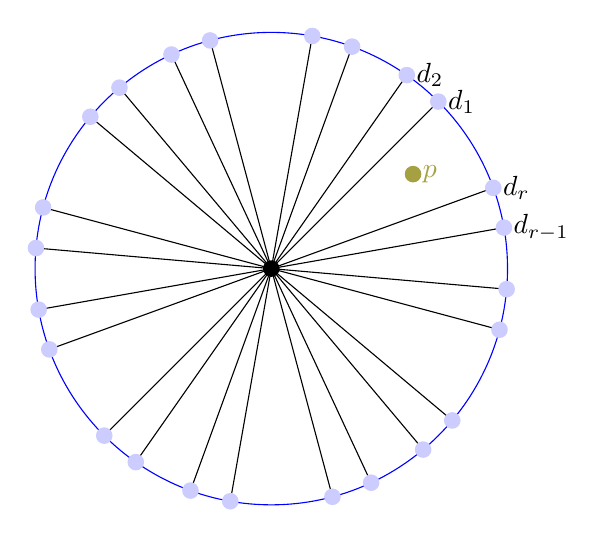
\begin{tikzpicture}[scale=3]
      \node[] (zero) at (0,0) {};
      \draw[blue] (zero) circle (1cm);

      \foreach \w/\str in {10/$d_{r-1}$,
                           20/$d_r$,
                           45/$d_1$,
                           55/$d_2$}
      {\draw (0,0) -- +({cos( \w )},{sin( \w )}) node[right] {\str};
       \fill[blue!20!white] ({cos( \w )},{sin( \w )}) circle (1pt);
       \foreach \sep in {60,120,180,240,300}
       {\draw (0,0) -- +({cos( \w + \sep )},{sin( \w + \sep )});
        \fill[blue!20!white]
          ({cos( \w + \sep )},{sin( \w + \sep )}) circle (1pt);
       }
      };

      \fill[yellow!60!black] (0.6,0.4) circle (1pt);
      \node[yellow!60!black,right] at (0.6,0.4) {$p$};

      \fill (zero) circle (1pt);
    \end{tikzpicture}
  \end{center}
  Label the first anti-Stokes ray when turning in a positive sense from $p$ as
  $d_1$ and label the subsequent rays $d_2,\dots,d_r$ in turn.
\end{frame}

\begin{frame}{Labeling convention (2): Sectors}
  \begin{center}
    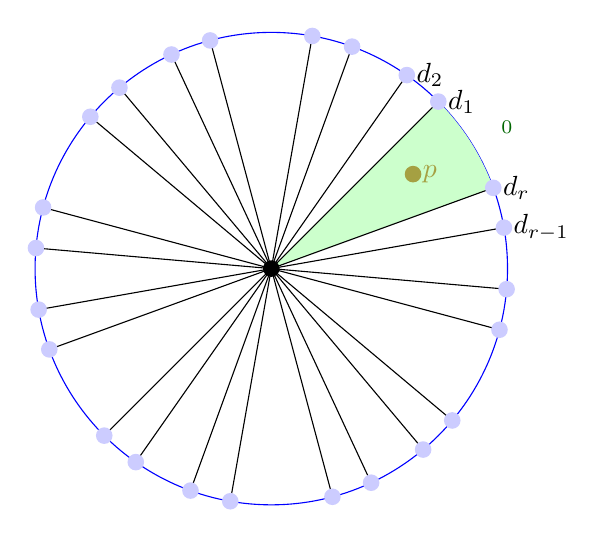
\begin{tikzpicture}[scale=3]
      \node[] (zero) at (0,0) {};
      \draw[blue] (zero) circle (1cm);

      \fill[fill=green!20!white] (0,0) -- ({cos( 20 )},{sin( 20 )}) arc
      (20:45:1) -- cycle;
      \node[green!40!black] at (1.0,0.6) {$\Sect_0$};

      \foreach \w/\str in {10/$d_{r-1}$,
                           20/$d_r$,
                           45/$d_1$,
                           55/$d_2$}
      {\draw (0,0) -- +({cos( \w )},{sin( \w )}) node[right] {\str};
       \fill[blue!20!white] ({cos( \w )},{sin( \w )}) circle (1pt);
       \foreach \sep in {60,120,180,240,300}
       {\draw (0,0) -- +({cos( \w + \sep )},{sin( \w + \sep )});
        \fill[blue!20!white]
          ({cos( \w + \sep )},{sin( \w + \sep )}) circle (1pt);
       }
      };

      \fill[yellow!60!black] (0.6,0.4) circle (1pt);
      \node[yellow!60!black,right] at (0.6,0.4) {$p$};

      \fill (zero) circle (1pt);
    \end{tikzpicture}
  \end{center}
  \begin{itemize}
    \item Write $\Sect_i:= \Sect(d_i,d_{i+1})$ the ‘ith sector’.
    \begin{itemize}
      \item Note $p \in\Sect_r= \Sect_0$
    \end{itemize}
  \end{itemize}
\end{frame}

\begin{frame}{Labeling convention (3): Supersectors}
  \begin{itemize}
    \item $\widehat{\Sect}_i:=
      \Sect(d_i-\frac{\pi}{2k-2},d_{1+1}+\frac{\pi}{2k-2})$ the ‘ith supersector’
      \begin{itemize}
        \item The rays bounding these supersectors are usually refered as
          \textcolor{red!40!black}{‘Stokes rays’}.
      \end{itemize}
  \end{itemize}
  \begin{center}
    \begin{tikzpicture}[scale=3]
      \node[] (zero) at (0,0) {};
      \draw[blue] (zero) circle (1cm);

      \fill[fill=green!20!white] (0,0) -- ({cos( 15 )},{sin( 15 )}) arc
        (15:85:1) -- cycle;

      \fill[fill=red!60!black] (0,0) -- ({cos( 15 )*0.5},{sin( 15 )*0.5}) arc
        (15:45:0.5) -- cycle;
      \fill[fill=red!60!black] (0,0) -- ({cos( 55 )*0.5},{sin( 55 )*0.5}) arc
        (55:85:0.5) -- cycle;

      \fill[fill=green!20!white] (0,0) -- ({cos( 15 )*0.4},{sin( 15 )*0.4}) arc
        (15:85:0.4) -- cycle;

      \node[green!40!black] at (.9,.9) {$\widehat\Sect_1$};

      \node[] (lft) at ({cos( 85 )},{sin( 85 )}) {};
      \node[] (rgt) at ({cos( 15 )},{sin( 15 )}) {};

      \draw[->,red!40!black] ({cos( 45 )},{sin( 45 )})
        to [out=35, in=25] (rgt);

      \draw[->,red!40!black] ({cos( 55 )},{sin( 55 )})
        to [out=65, in=75] (lft);

      \draw[thick,red!40!black,path fading=west] (0,0) -- +({cos( 85 )},{sin( 85 )});
      \draw[thick,red!40!black,path fading=west] (0,0) -- +({cos( 15 )},{sin( 15 )});
      \fill[red!40!black] ({cos( 85 )},{sin( 85 )}) circle (1pt);
      \fill[red!40!black] ({cos( 15 )},{sin( 15 )}) circle (1pt);

      \foreach \w/\str in {10/$d_{r-1}$,
                           20/$d_r$,
                           45/$d_1$,
                           55/$d_2$}
      {\draw (0,0) -- +({cos( \w )},{sin( \w )}) node[right] {\str};
       \fill[blue!20!white] ({cos( \w )},{sin( \w )}) circle (.7pt);
       \foreach \sep in {60,120,180,240,300}
       {\draw (0,0) -- +({cos( \w + \sep )},{sin( \w + \sep )});
        \fill[blue!20!white]
          ({cos( \w + \sep )},{sin( \w + \sep )}) circle (.7pt);
       }
      };

      \fill[yellow!60!black] (0.6,0.4) circle (1pt);
      \node[yellow!60!black,right] at (0.6,0.4) {$p$};

      \fill (zero) circle (1pt);
    \end{tikzpicture}
  \end{center}
\end{frame}
\begin{frame}{Labeling convention (4)}
  All \textcolor{red!40!black}{‘Stokes rays’}:
  \begin{center}
    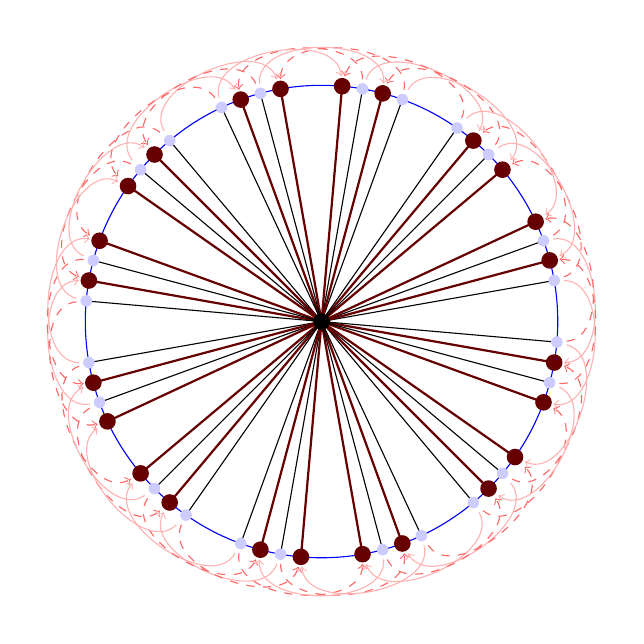
\begin{tikzpicture}[scale=3]
      \node[] (zero) at (0,0) {};
      \draw[blue] (zero) circle (1cm);

      \foreach \w/\str in {10/,
                           20/,
                           45/,
                           55/}
      {\draw (0,0) -- +({cos( \w )},{sin( \w )}) node[right] {\str};
       \fill[blue!20!white] ({cos( \w )},{sin( \w )}) circle (.7pt);

       \foreach \sep in {0,60,120,180,240,300}
       {\node[] (src) at ({cos( \w + \sep )},{sin( \w + \sep)}) {};
        \node[] (lft) at ({cos( \w + \sep + 30 )},{sin( \w + \sep + 30 )}) {};
        \node[] (rgt) at ({cos( \w + \sep - 30 )},{sin( \w + \sep - 30 )}) {};
        \draw[thick,red!40!black] (0,0)
          -- +({cos( \w + \sep + 30 )},{sin( \w + \sep + 30 )});
        %\draw[thick,red!40!black] (0,0)
          %-- +({cos( \w + \sep - 30 )},{sin( \w + \sep - 30 )});

        \draw[->,red!30!white] (src)
          to [out={\w + \sep - 10}, in={\w + \sep - 30 + 10}] (rgt);
        \fill[red!40!black] (rgt) circle (1pt);

        \draw[->,red!60!white,dashed] (src)
          to [out={\w + \sep + 10}, in={\w + \sep + 30 - 10}] (lft);
       }
       \foreach \sep in {60,120,180,240,300}
       {\draw (0,0) -- +({cos( \w + \sep )},{sin( \w + \sep )});
        \fill[blue!20!white]
          ({cos( \w + \sep )},{sin( \w + \sep )}) circle (.7pt);
       }
      };

      \fill (zero) circle (1pt);
    \end{tikzpicture}
  \end{center}
\end{frame}
%}}}
%%%%%%%%%%%%%%%%%%%%%%%%%%%%%%%%%%%%%%%%%%%%%%%%%%%%%%%%%%%%%%%%%%%%%%%%%%%%%%%

%%%%%%%%%%%%%%%%%%%%%%%%%%%%%%%%%%%%%%%%%%%%%%%%%%%%%%%%%%%%%%%%%%%%%%%%%%%%%%%
\section{Local Moduli and the Stokes phenomenon}%%%%%%%%%%%%%%%%%%%%%%%%%%%%{{{
\begin{frame}[t]
  {\Huge\insertsection{}}
  \begin{itemize}
    \item \cite{boalch}
  \end{itemize}
  and
  \begin{itemize}
    \item \cite{Loday1994}
  \end{itemize}
\end{frame}

\begin{frame}{Now we move on to the local moduli of meromorphic connections}
$\Syst(A^0):=\{d-A \mid A=\hat{F}[A^0] \text{ for some } \hat{F}\in
  G\llbracket z\rrbracket\}$\footnote{the set of germs at $0\in\C$ of
  meromorphic connections on the trivial rank $n$ vector bundle, that are
  formally equivalent to $d-A^0$.}
where
  \begin{itemize}
    \item $A$ is a matrix of germs of meromorphic one-forms
    \item $\hat{F}[A^0]=(d\hat{F})\hat{F}^{-1}+\hat{F}A^0\hat{F}^{-1}$
    \item $G\llbracket z\rrbracket:=\GL_n(\C\llbracket z\rrbracket)$
      \begin{itemize}
        \item does not act on $\Syst(A^0)$
      \end{itemize}
  \end{itemize}
  The group $G\{z\}:=\GL_n(\C\{z\})$ acts on $\Syst(A^0)$,  study
  \begin{center}
    $\Syst(A^0)/G\{z\}$\footnote{The set of isomorphism classes of germs of
    meromorphic connections formally equivalent to $A^0$. Note that any generic
    connection is formally equivalent to some such $A^0$.}
  \end{center}
  In the abelian and the simple pole case this is only a point.
\end{frame}

\begin{frame}{It is useful to consider spaces slightly larger than $\Syst(A^0)$}
  \begin{itemize}
    \item $\widehat\Syst_{cf}(A^0)$ :\Leftrightarrow the set of compatibly
      framed connection germs with both irregular and formal type $A^0$.
    \item $\widehat\Syst_{mp}(A^0):=\{(A,\hat{F})\mid A\in\Syst(A^0)
      ,\hat{F}\in G\llbracket z\rrbracket
      ,A=\hat{F}[A^0]\}$
      the set of \emph{marked pairs}.
  \end{itemize}
  There is a canonical isomorphism
  $\widehat\Syst_{cf}(A^0)\cong\widehat\Syst_{mp}(A^0)$\footnote{Let
  $\Syst(A^0)$ denote either of these two sets.}.

  $G\{z\}$ action on marked pairs: $g(A,\hat{F})=(g[A],g\circ\hat{F})$
  \[
    \mathcal{H}(A^0):=\widehat\Syst(A^0)/G\{z\}
  \]
  Moreover the actions of $T$ and $G\{z\}$ on $\Syst(A^0)$ commute so
  \[
    \Syst(A^0)/G\{z\}\cong\mathcal{H}(A^0)/T
  \]
\end{frame}

\begin{frame}
  \begin{thm}[1.22 in \cite{thboalch}]
    There is a natural isomorphism
    \[
      \cH(A^0)\cong\prod_{d\in\A}\Sto_d(A^0)
    \]
    and for each choice of $\log(z)$ in the direction $d$ the Stokes group
    $\Sto_d(A^0)$ has a faithfull representation $\rho$ on $\C^n$ inducing an
    isomorphism
    \[
      \rho:\Sto_d(A^0)\to\SSto_d(A^0).
    \]
    In particular each $\Sto_d(A^0)$ and therefore $\cH(A^0)$ is a\dots
  \end{thm}
\end{frame}

\begin{frame}{Theorem 3.1}
  \begin{thm}[3.1, or Prop 1.24 in \cite{thboalch}]
    Let $\hat{F}\in G\llbracket z\rrbracket$1 such that $A:=F[A_0]$ has
    convergent entries.
    Set the radius of the sectors $\Sect_i$, $\widehat\Sect_i$ to be less than
    the radius of convergence of $A$.
    Then:
    \begin{enumerate}
      \item On each sector $\Sect_i$ there is a canonical way to choose an
        invertible $n\times n$ matrix of holomorphic Functions
        $\Sigma_i(\hat F)$ such that $\Sigma_i(\hat F)[A^0]=A$
      \item $\Sigma_i(\hat F)$ can be analytically continued to the supersector
        $\widehat\Sect_i$ and then $\Sigma_i(\hat F)$ is asymptotic to $\hat F$
        at $0$ within $\widehat\Sect_i$
      \item If $g\in G\{z\}$ and $t\in T$ then
        $\Sigma_i(g\circ\hat F \circ t^{-1})=g\circ\Sigma_i(\hat F)\circ t^{-1}$.
    \end{enumerate}
  \end{thm}
  \begin{itemize}
    \item The point is that on a narrow sector there are generally many
      holomorphic isomorphisms between $A_0$ and $A$ which are asymptotic to
      $\hat F$ and one is being chosen in a canonical way
    \item $\Sigma_i(\hat F)$ is in fact uniquely characterised by property 2.
  \end{itemize}
  \begin{prop}[Prop 1.24 in \cite{thboalch}]
    \begin{enumerate}
    \setcounter{enumi}{2}
    \item If $\hat H\in\hat G$ is the taylor series at $0$ of an analytic gauge
      transformation $H\in G\{z\}$ then
      \[
        \Sigma_i(\hat H \hat F)=H\Sigma_i(\hat F)
        \qquad
        \Sigma_i(\hat F \hat H)=\Sigma_i(\hat F)H
      \]
  \end{enumerate}
  \end{prop}
\end{frame}

\begin{frame}{Functions on the quotient $\mathcal{H}(A^0)$}
  Let
  \begin{itemize}
    \item $(A,g_0)\in\widehat\Syst(A^0)$ be a compatibly framed connection germ
    \item $\hat F\in G\llbracket z\rrbracket$ be the associated  formal
      isomorphism
  \end{itemize}
  The sums of $\hat F$ on the two sectors andjacent to some anti-Stokes ray
  $d_i$ may be analytically continued across $d_i$ and they generally be
  different on the overlap.
  Thus for each anti-Stokes ray $d_i$ there is a matrix of holomorphic
  functions
  \[
    \kappa_i:=\Sigma_i(\hat F)^{-1}\circ\Sigma_{i-1}(\hat F)
  \]
  asymptotic to $i$ on a sectorial neighbourhood of $d_i$.

  Moreover \textcolor{red!60!black}{clearly} $\kappa_i[A^0]=A^0$.

  A concrete description of $\kappa_i$ is obtained by choosing a basis of
  solution of $A^0$, which is made via a choice of branch of $\log(z)$.
\end{frame}
\begin{frame}{Remark in \cite{thboalch}}
  \begin{rem}[1.41 from \cite{thboalch} on pages 16f]
    Note that in most of the recent references we have used, Stokes matrices
    are used to classify
    \begin{itemize}
      \item meromorphic connections within fixed formal \textbf{meromorphic
        classes, modulo meromorphic equivalence}.
    \end{itemize}
    Whereas here we classify
    \begin{itemize}
      \item meromorphic connections within fixed \textbf{formal analytic
        classes, modulo analytic equivalence},
    \end{itemize}
    as is done in the older literature.  The fact is that the sets equivalence
    classes are the same in both cases. It is important for us to work with
    analytic, rather than meromorphic gauge transformations, because then the
    $\C^\infty$ viewpoint in Chapter 3 is cleaner. This distinction relates to
    the difference between \textbf{‘regular singular’} connections and
    \textbf{‘logarithmic’} connections.
  \end{rem}
\end{frame}
%}}}
%%%%%%%%%%%%%%%%%%%%%%%%%%%%%%%%%%%%%%%%%%%%%%%%%%%%%%%%%%%%%%%%%%%%%%%%%%%%%%%

%%%%%%%%%%%%%%%%%%%%%%%%%%%%%%%%%%%%%%%%%%%%%%%%%%%%%%%%%%%%%%%%%%%%%%%%%%%%%%%
\section{Asymptotic expansions}%%%%%%%%%%%%%%%%%%%%%%%%%%%%%%%%%%%%%%%%%%%%%{{{
\begin{frame}[t]
  {\Huge\insertsection{}}
  \begin{itemize}
    \item \cite{sabbah_cimpa90} §2.2.2 Asymptotic expansions
    \item \cite{van2003galois} Chap. 7 Exact Asymptotics
  \end{itemize}
  and
  \begin{itemize}
    \item \cite{majima1984asymptotic}
    \item \cite{zbMATH00060600}
    \item \cite{wasow2002asymptotic}
  \end{itemize}
\end{frame}

\begin{frame}{Another definition of sectors}
  Let \textcolor{red!60!black}{$U$} be an open interval in $S^1$
  \begin{itemize}
    \item $\Delta_r^*(U):=
      \{z\in\Delta_r\mid z=\rho e^{i\theta},0<\rho<r,\theta\in U\}$%
    \begin{center}
      \begin{tikzpicture}[scale=3]
        \node (zero) at (0,0) {};
        \node[below left] at (zero) {$0$};
        \draw[blue,dashed] (zero) circle (1cm);

        \filldraw[fill=green!20!white
                 ,draw=green!60!black
                 ,thick
                 ,path fading=west] (0,0)
          -- ({cos( -30 )*.7},{sin( -30 )*.7}) arc (-30:70:.7) -- cycle;
        \node[green!40!black] at (.4,.3) {$\Delta_r^*(U)$};
        \node[green!40!black] at (.3,-.25) {$r$};

        \draw[thick,red!60!black] ({cos( -30 )},{sin( -30 )}) arc (-30:70:1);

        \node[red!60!black,right] at (1,0) {$U$};

        \fill[white] (zero) circle (1.5pt);
        \fill (zero) circle (.7pt);
      \end{tikzpicture}
    \end{center}
    \item $\Delta_r:=\Delta_r^*(S^1)$
  \end{itemize}
\end{frame}

\begin{frame}{Asymptotic expansion}
Let $\hat\phi=\sum_{n\geq-n_0}a_nx^n$ with $a_n\in\C$ is as asymptotic
expansion of $f$ at $0$ if for all $m\in\N$ one has
\begin{equation} \label{eq:asymptoticExpansion}
  \lim_{x\to 0,x\in\triangle_r^*(U)}
  \left|x^{-m}\right|\left|x^{n_{0}}f(x)-\sum_{0\leq n\leq m}a_{n}x^{n}\right|
  =0
\end{equation}
Define
\begin{itemize}
  \item $\bar\cA(U,r)\subset\cO(\Delta_r^*(U))$ the set of functions which
    admits an asymptotic power series
  \item $\cA(U,r):=\bigcap_{V}\bar\cA(V,r)$ where $V$ are relatively
    compact open subsets of $U$
    \begin{itemize}
      \item $\cA(U,r)=\{\phi\in \bar\cA(U,r)
        \mid \phi\in \bar\cA(V,r)
        \forall V\text{ rel.\  cp.\  op.\  subset of }U\}$
    \end{itemize}
  \item $\cA(U):=\bigcup_r\cA(U,r)$%
    \begin{itemize}
      \item $\cA(U)=\{\phi\mid\exists r\text{: } \phi\in\cA(U,r)\}
        =\{\phi\mid\exists r\text{: }
          \forall V\subset U\text{ rel.cp.op.}\text{: }
          \phi\in\bar\cA(V,r)\}$
    \end{itemize}
\end{itemize}
The mapping $U\mapsto\cA(U)$ defines a sheaf on $S^1$
\end{frame}

\begin{frame}
\begin{probl}
\begin{itemize}
  \item are there any restrictions to the coefficients $a_{-n_0},\dots,a_{-1}$?
\end{itemize}
\end{probl}
Take a look at $f=\frac{1}{x}$ and restrict to $\theta=0$ ($\R_{>0}$), then:
\[
  \forall m : \qquad
  \lim_{x\to 0,x\in\R_{>0}}
  \left|x^{-m}\right|\left|\frac{x^{n_{0}}}{x}
    -\sum_{0\leq n\leq m}a_{n}x^{n}\right| =0
\]
In the case $m=0$ we get $\left|\frac{x^{n_{0}}}{x} -a_{0}\right|\to0$. This
implies $n_0\geq1$, lets take $n_0=1$ and $a_0=1$.

In the case $m=1$ we get
$\frac{\left|\frac{x}{x} -1 -a_1x\right|}{|x|}\to0$

Thus
$ \left|\frac{x}{x^2} -\frac{1}{x} -a_1\right|\to0 $

Thus
$ \left|\frac{1}{x} -\frac{1}{x} -a_1\right|\to0$ Thus $a_1=0$ and so on
\end{frame}

{\setbeamercolor{background canvas}{bg=gray!40!white}
  \begin{frame}[t]{Definition from \cite{van2003galois} (!!)}
    Let $f$ be a holomorphic function on $S(a,b,\rho)$, where
    \begin{itemize}
      \item $a,b\in S^1=\R/2\pi\Z$ and
      \item $\rho$
        \begin{itemize}
          \item is a continous function on the open interval $(a,b)$ and
          \item has values in the positive real numbers
        \end{itemize}
        and
      \item $S(a,b,\rho)$ are the complex numbers $z\neq0$ satisfying
        \begin{itemize}
          \item $\arg(z)\in(a,b)$ and
          \item $|z|<\rho(\arg(z))$.
        \end{itemize}
    \end{itemize}
    \begin{defn}[7.1]
      \def\myN{\textbf{\textcolor{blue!40!black}{N}}}
      \def\mySect{\textcolor{red!40!black}{W}}
      \def\myConst{\textcolor{green!40!black}{C(\myN,\mySect)}}
      $f$ has the \textbf{formal Laurent series} $\sum_{n\geq n_0}c_nz^n$ as
      asymptotic expansion if
      \begin{itemize}
        \item for every $\myN\geq0$ and
        \item every closed subsector $\mySect$ in $S(a,b,\rho)$
      \end{itemize}
      there exists a constant $\myConst$ such that
      \[
        \left|
          f(x)-\sum_{n_0\leq n\leq \myN-1}c_nz^n
        \right|
        \leq \myConst|z|^{\myN} \qquad \text{ for all } z\in \mySect
      \]
      \Leftrightarrow{}
      \[
        \lim_{z\to0,z\in{\mySect}}
        |z|^{-(\myN-1)}
        \left|
          f(x)-\sum_{n_0\leq n\leq \myN-1}c_nz^n
        \right|=0
        \qquad \text{ for all } z\in \mySect
      \]
    \end{defn}
    \begin{itemize}
      \item One writes $J(f)$ for the formal Laurent series.
      \item Define $\cA(a,b)$ as the limit of the $\cA(S(a,b,\rho))$ where
        \begin{itemize}
          \item $\cA(S(a,b,\rho))$ are the functions with asymptotic expansion.
        \end{itemize}
    \end{itemize}
  \end{frame}

  \begin{frame}[t]{Definition from \cite{van2003galois} (1)}
    \begin{defn}[7.4]
      Let
      \begin{itemize}
        \item $k$ be a positive real number and
        \item $S$ be an open sector.
      \end{itemize}
      A function $f\in\cA(S)$, with asymptotic expansion
      $J(f)=\sum_{n\geq n_0}c_nz^n$, is said to bea a \emph{Grevrey function of
      order $k$} if:
      \\For every closed subsector $W$ of $S$ there are constants
      \begin{itemize}
        \item $A>0$ and
        \item $c>0$
      \end{itemize}
      such that for all
      \begin{itemize}
        \item $N\geq1$ and
        \item all $z\in W$ and $|z|\leq c$
      \end{itemize}
      one has
      \[
        \left| f(z)-\sum_{n_0\leq n\leq N-1}c_nz^n \right| \leq
        A^N \textcolor{green!40!black}{\Gamma\left(1+\frac{N}{k}\right)}|z|^N
      \]
      or equivalently
      \[
        \left| f(z)-\sum_{n_0\leq n\leq N-1}c_nz^n \right|
        \leq A^N \textcolor{green!40!black}{(N!)^{\frac{1}{k}}} |z|^N
      \]
    \end{defn}
  \end{frame}

  \begin{frame}[t]{Definition from \cite{thboalch}, Appendix C}
    Let
    \begin{itemize}
      \item $f$ be a holomorphic function on $S$, where
        \begin{itemize}
          \item $S:=\{z\in\C\mid\alpha<\arg(z)<\beta, 0<|z|<r\}$
        \end{itemize}
        and
      \item $\hat f=\sum_{n\geq0}a_nz^n\in \C\llbracket z\rrbracket$ be an
        arbitrary formal power series
    \end{itemize}
    \begin{defn}[C.1]
      The function $f$ is said to \emph{have asymptotic expansion $\hat f$ on
      $S$} if,
      \begin{itemize}
        \item for each closed subsector $S'\subset S$
        \item and integer $p$,
      \end{itemize}
      there is a constant $c\in\C$ such that
      \[
        \left|f(z)-\sum_{n=0}^pa_nz^n\right|\leq c|z|^{p+1}
      \]
    \end{defn}
    One way of think of this condition is \textbf{in terms of convergence of
    the derivatives of $f(z)$:}
    if $f$ is holomorphic on $S$ then it t urns out that $f$ has asymptotic
    expansion $\hat f$ on $S$ iff for each closed subsector $S'\subset S$ and
    integer $n$ we have
    \[
      \underset{s\in S'}{\lim_{z\to0}} f^{(n)}=n!a_n
    \]
  \end{frame}

  \begin{frame}[t]{Definition from \cite{zbMATH00060600}}
  \begin{defn}
    $f=\sum_ma_mx^m$ is of \emph{Grevrey order $s$} (nonegative)
    :\Leftrightarrow
    \begin{itemize}
      \item there exist $C$ and $A$ nonegative such that
      \[
        |a_m|< C(m!)^sA^m \qquad \text{ for } m=0,1,2,\dots
      \]
    \end{itemize}
    We denote by $\C\llbracket z\rrbracket_s$ the set of all power series of
    Grevrey order $s$.
  \end{defn}
  \begin{defn}
  $\phi$ is said to admit an asymptotic expansion of Grevrey order $s$ as
  $z\to0$ on
  \[
    \mathcal{D}(R_0,a,b):=\{z \mid a < \arg z < b , 0 < |z| < R_0\}
  \]
  if
  \begin{itemize}
    \item $\phi$ is holomorphic on $\mathcal{D}(R_0,a,b)$
    \item there exists a formal power series
    $f=\sum_{m\geq0}a_mz^m \in \C\llbracket z\rrbracket_s$ such that
    \[
      \left|\phi(z)-\sum_{N-1\geq m\geq 0}a_mz^m\right|
      \leq K_{R,\alpha,\beta}(N!)^s(B_{R,\alpha,\beta})^N|z|^N
    \]
    on $\mathcal{D}(R,\alpha,\beta)$ for $N=1,2,\dots$ and every
    $(R,\alpha,\beta)$ satisfying
    \[
      0 < R < R_0 \qquad \text{ and } \qquad a < \alpha < \beta < b,
    \]
    where $K_{R,\alpha,\beta}$ and $B_{R,\alpha,\beta}$ are some nonegative
    numbers depending on $(R,\alpha,\beta)$.
  \end{itemize}
  \end{defn}
  \end{frame}

  \begin{frame}[t]{Definition from \cite{zbMATH00060600} (2)}
    \begin{itemize}
      \item We denote by $\mathcal{A}_s(R_0,a,b)$ the set of all functions
      admitting asymptotic expansions of Grevrey $s$ as $z\to 0$ on the
      sectorial domain $\mathcal{D}(R_0,a,b)$.
      \item We set $J(\phi)=f$. Then the mapping
      \[
      J: \mathcal{A}_s(R_0,a,b) \to \C\llbracket z\rrbracket_s
      \]
      is a homomorphism of commutative differential algebras over $\C$.
      \item Set
      \[
      \mathcal{A}_{s,0}(R_0,a,b):=
      \ker\left(J: \mathcal{A}_s(R_0,a,b) \to \C\llbracket z\rrbracket_s\right)
      \]
    \end{itemize}
    \begin{lem}[1.3]
      A function $\phi(z)$ belongs to $\mathcal{A}_{s,0}(R_0,a,b)$ iff \dots
    \end{lem}
    \begin{cor}[1.4]
      $J$ is injective iff \dots
    \end{cor}
    \begin{defn}[1.5]
      Let $k$ be a positive number. A formal power series $f\in\C\llbracket
      z\rrbracket$ is \emph{k-summable in a direction} $\arg z=d$\dots
    \end{defn}

    \dots

    \textbf{2. Grevrey properties of formal solutions:} We can define the
    Newton polygon\dots
  \end{frame}

  \begin{frame}[t]{Other definitions}
    \begin{itemize}
      \item \textbf{\cite[2]{majima1984asymptotic} says:}
        \\$f\in\cA(U)$ iff for every \textbf{closed} subsector and for every
        $N\in\N$
        \[
          \sup_{x\in\bar\cA(V,\tilde r)}
            \left|x^{-N}\left(f(x)-\sum_{i=0}^{N-1}a_ix^i\right)\right|
          <+\infty
        \]
      \item \textbf{\cite{wasow2002asymptotic} defines:}
        \\Let the function $f(x)$ be defined in a point-set $S$ of the complex
        $x$-plane having $x=0$ as an accumulation point. The power series
        $\sum_{r=0}^\infty a_rx^r$ is said to represent $f(x)$ asymptotically,
        as $x\to0$ is $S$, if
        \[
          x^{-m}\left[f(x)-\sum_{r=0}^ma_rx^r\right]
        \]
        tends to zero, for all $m\geq0$, as $x$ tends to zero in $S$.
    \end{itemize}
  \end{frame}
}

\begin{frame}{Some elementary properties (2.2.4)}
  \begin{enumerate}
    \item If $\hat\phi$ is an Asymptotic expansion for $f$ then one has
      \[
        a_0=\lim_{x\to 0,x\in\Delta_r^*(U)}x^{n_0}f(x)
      \]
      and for $m>0$,
      \[
        a_m=\lim_{x\to 0,x\in\Delta_r^*(U)}x^{-m}
          \left[x^{n_0}f(x)-\sum_{0\leq n\leq m-1}a_nx^n\right]
      \]
      In particular this asymptotic expansion is unique
      \begin{itemize}
        \item $f$ admits a zero asymptotic expansion iff for all $p\in\Z$
          one has
          \[
            \lim_{x\to 0,x\in\Delta_r^*(U)}x^pf(x)=0
          \]
      \end{itemize}
    \item
      Define $\cA(U)\to \hat K$ denoted by $f\mapsto \hat{f}$.
      \begin{itemize}
        \item $\cA(U)$ is a subring of $\cO(\Delta_r^*(U))$
        \item this mapping is a morphism of rings
      \end{itemize}
    \item Denote by $\cA^{<0}(U)$ the kernel of this morphism
      \begin{itemize}
        \item $x\mapsto e^{-\frac{1}{x}}$ has zero asymptotic expansion in
          some sector around $\theta=0$
      \end{itemize}
    \item $\cA(U)$ is stable under derivation\footnote{Proof in
      \cite{sabbah_cimpa90}}.
    \item $\cA(U)$ contains $K$ as a subfield.
  \end{enumerate}
\end{frame}

\begin{frame}{Borel-Ritt lemma}
  \begin{lem}[2.2.5]
  If $U$ is a proper open interval of the unit circle the mapping
  \[
  \cA(U)\to\hat{K}
  \]
  is onto\footnote{1p proof at~\cite{sabbah_cimpa90}[p63]}.
  \end{lem}

  It follows from this lemma that one has an exact sequence
  \[
    0 \to \cA^{<0}(U) \to \cA(U) \to \hat{K} \to 0 \,.
  \]
\end{frame}
%}}}
%%%%%%%%%%%%%%%%%%%%%%%%%%%%%%%%%%%%%%%%%%%%%%%%%%%%%%%%%%%%%%%%%%%%%%%%%%%%%%%
%%%%%%%%%%%%%%%%%%%%%%%%%%%%%%%%%%%%%%%%%%%%%%%%%%%%%%%%%%%%%%%%%%%%%%%%%%%%%%%
\section{Asymptotic expansions: Main result}%%%%%%%%%%%%%%%%%%%%%%%%%%%%%%%%{{{
\begin{frame}[t]
  {\Huge\insertsection{}}
  \begin{itemize}
    \item \cite{sabbah_cimpa90} §2.2.3
  \end{itemize}

  \begin{thm}[2.3.1]
    Let $\cM_K$ be a meromorphic connection. There exists an integer $q\geq 1$
    such that, after the ramification $x=t^q$, one has, for all $\theta\in S^1$
    and each sufficiently small interval $V$ centered at $\theta$
    \[
      \cA_L(V)\otimes_L\cM_L \cong
        \cA_L(V)\otimes_L\left(\cF_L^R\otimes\cG_L\right)
    \]
  \end{thm}
\end{frame}

\begin{frame}[t]{Corollaries}
  For all $\theta\in S^1$ and each \textbf{sufficiently small interval $U$}
  centered
  at $\theta$:
  \begin{cor}[2.3.2]
    Let $\cM_K$ be a meromorphic connection.
    The formal decomposition into one slope terms
    $\cM_{\hat K}=\bigoplus \cM_{\hat K}^{L_i}$ can be liftet into a
    decomposition
    \[
      \cA(U)\otimes_K\cM_K \cong \bigoplus\cM_{\cA(U)}^{L_i}
    \]
  \end{cor}
  \begin{cor}[2.3.3]
    Let
    \begin{itemize}
      \item $\cM_K$ and $\cM_K'$ be two meromorphic connections and
      \item $\hat\phi:\cM_{\hat{K}}\to\cM_{\hat{K}}'$ a left
        $\cD_{\hat K}$-linear \textcolor{green!40!black}{(iso-)}morphism.
    \end{itemize}
    Then
    $\hat\phi$ can be liftet into a $\cD_{\cA(U)}$-linear
    \textcolor{green!40!black}{(iso-)}morphism
    \[
      \phi_U:\cA(U)\otimes_K\cM_K\to\cA(U)\otimes_K\cM_K'
    \]

    \begin{lem}[2.3.4]
      Let $\cN_K$ be a meromorphic connection.
      The natural\footnote{Induced by the Borel-Ritt lemma?} mapping
      \[
        \ker\left[\partial_x:\cN_{\cA(U)}\to\cN_{\cA(U)}\right]
        \to
        \ker\left[\partial_x:\cN_{\hat K}\to\cN_{\hat K}\right]
      \]
      is onto.
    \end{lem}
  \end{cor}
\end{frame}

\begin{frame}[t]{Proof (2.3.1)}
  Let $\cM_K$ be a meromorphic connection. Choose first a ramified covering
  $t\mapsto x=t^q$ in order to apply theorem I-5.4.7:
  \[
    \cM_{\hat L}\cong\bigoplus\cF_{\hat L}^R\otimes\cG_{\hat L}
  \]
  \begin{thm}[I-5.4.7]
    Let $\cM_{\hat K}$ be a formal meromorphic connection. There exists an
    integer $q$ sucht that the connection $\pi^*\cM_{\hat K}=\cM_{\hat L}$ is
    isomorphic to a direct sum of elementary formal meromorphic connections.
    \begin{defn}[5.4.4 + 5.4.5]
      Let $R(z)=\sum_{i=1}^ka_iz^i\in\C[z]_k$.
      \begin{itemize}
        \item We shall denote by $\cF_{\hat K}^R$ the following meromorphic
          connection:
          \begin{itemize}
            \item The $\hat K$-vector space is isomorphic to $\hat K$ with a
              basis denoted by $e(R)$.
            \item
              The action of $x\partial_x$ is defined
              by
              \[
                x\partial_x(\phi\cdot e(R))=\left[
                  x\frac{\partial\phi}{\partial x}
                  +\phi x\frac{\partial R(x^{-1})}{\partial x}
                \right]\cdot e(R)
              \]
          \end{itemize}
        \item An \emph{elementary meromorphic connection} (over $\hat K$) is a
          connection isomorphic to $\cF_{\hat K}^R\otimes_{\hat K}\cG_{\hat K}$
          where
          \begin{itemize}
            \item $\cG_{\hat K}$ is an elementary regular meromorphic
              connection.
          \end{itemize}
      \end{itemize}
    \end{defn}
  \end{thm}
\end{frame}

\begin{frame}[t]{Proof (2.3.1)}
  Put $\cM_{\hat L}=\cM_{\hat L}'\oplus\cM_{\hat L}''$ where
  \begin{itemize}
    \item $\cM_{\hat K}'$ is the sum of terms
      $\cF_{\hat L}^R\otimes\cG_{\hat L}$ for which
      \begin{itemize}
        \item $R$ has maximal degree $k$ and
        \item with fixed dominating coefficient $\alpha\in\C$
      \end{itemize}
    \item $\cM_{\hat K}''$ the sum of the other terms.
  \end{itemize}
  The proof will be done \textbf{by induction}, by showing that this splitting
  can be liftet to $\cA_{L}(V)$ when $V$ is sufficiently small.  However the
  terms $\cM_{\cA_{L}(V)}'$ and $\cM_{\cA_{L}(V)}''$ do not come necessarily
  from modules defined over $L$.\footnote{That is why the proof has to be done
  for modules defined over $\cA_{L}(V)$.}
  \begin{lem}[2.4.1]
    \begin{itemize}
      \item Let $\cM_{\cA_L(V)}$ be a free $\cA_L(V)$-module equipped with a
        connection and
      \item let $\cM_{\hat L}$ be its formalized module.
    \end{itemize}
    A splitting of $\cM_{\hat L}$ as above can be lifted to a splitting of
    $\cM_{\cA_L(V)}$ when $V$ is sufficiently small.
  \end{lem}
\end{frame}

\begin{frame}[t]{Proof (2.3.1)}
  For the proof of (2.4.1):
  \\The first step is the case where $\cM_{\hat L}$ is regular. One must prove
  a result analogous to theorem I-5.2.2\footnote{\begin{lem}[I-5.2.2]
      Let $\cM_{\hat K}$ be regular formal meromorphic connection. Then there
      exist a basis for which the matrix $x\partial_x$ is constant.
    \end{lem}}:
  \begin{lem}[2.4.2]
    Let $\cM_{\cA_L(V)}$ be a free $\cA_L(V)$-module equipped with a connection
    such that $\cM_{\hat L}$ is regular.
    There exists a $\cA_L(V)$-basis $\textbf{m}$ of $\cM_{\cA_L(V)}$ such that
    the matrix of $t\partial_t$ in this basis is constant.
  \end{lem}

  We want to use:
  \begin{itemize}
    \item matrix of $t\partial_t$ is constant \Rightarrow{} there exists a
      basis $\textbf{m}$ such that the \textcolor{green!40!black}{corresponding
      basis $\hat{\textbf{m}}$} is compatible with the splitting of
      $\cM_{\hat L}$?
  \end{itemize}
\end{frame}
%}}}
%%%%%%%%%%%%%%%%%%%%%%%%%%%%%%%%%%%%%%%%%%%%%%%%%%%%%%%%%%%%%%%%%%%%%%%%%%%%%%%
\fi{} %}}}
%%%%%%%%%%%%%%%%%%%%%%%%%%%%%%%%%%%%%%%%%%%%%%%%%%%%%%%%%%%%%%%%%%%%%%%%%%%%%%%
\section{Sabbas sheaf view: Stokes sheaf}%%%%%%%%%%%%%%%%%%%%%%%%%%%%%%%%%%%{{{
\begin{frame}[t]
  {\Huge\insertsection{}}
  \begin{itemize}
    \item \cite{sabbah2007isomonodromic} \textbf{II.6:}
      The Riemann-Hilbert correspondence in the irregular case
  \end{itemize}

  \textcolor{green!60!black}{%
    The data which enable us to recover the meromorphic bundle with connection
    from the formal meromorphic bun- dle with connection are called a
    \emph{Stokes structure.}\footnote{It is in fact a sheaf on the parameter
    space.}
  }

  Three approaches to the stokes phenomenon:
  \begin{itemize}
    \item define the ``wild'' fundamental group and identify the category of
      meromorphic connections to that of the finite dimensional linear
      representations of this group
    \item identify the category of meromorphic connection to that of filtered
      local systems
    \item the theory of \textbf{multiplicity}
      \begin{itemize}
        \item enables one to analyze in a finer way
      \end{itemize}
  \end{itemize}
\end{frame}

\begin{frame}[t]{Holomorphic / Meromorphic bundles}
  \begin{defn}[Holomorphic budles (0.3.?)]
    Let
    \begin{itemize}
      \item $\pi:E\to M$ be a holomorphic mapping between two complex analytic
        manifolds.
    \end{itemize}
    We will say that
    \begin{itemize}
      \item $\pi$ is a \emph{vector fibration of rank $d$}, or
      \item $\pi$ makes $E$ a \emph{vector bundle of rank $d$ on $M$}
    \end{itemize}
    if there exists a open covering\dots
  \end{defn}
  Set $\sE(U)$ as the set of holomorphic sections, where
  \begin{itemize}
    \item a \emph{holomorphic section} of $E$ on $U$ is a holomorphic mapping
      $\sigma:U\to E$ which
      \begin{itemize}
        \item is a section of the projection, i.e., which satisfies
          $\pi\circ\sigma=\Id_U$.
      \end{itemize}
  \end{itemize}
  This defines a sheaf $\sE$ of modules over $\cO_M(U)$.
  \begin{prop}[Equivalence between vector bundles and locally free sheaves
    (0.4.1)]
  \end{prop}

  \begin{defn}[Meromorphic bundles (0.8.?)]
    A \emph{meromorphic bundle on $M$ with poles along $Z$} is a locally free
    sheaf of $\cO_M(*Z)$-modules of finite rank.
  \end{defn}
\end{frame}

\begin{frame}[t]{Holomorphic connections (0.11)}
  \begin{defn}[Holomorphic connections (0.11.1)]
    A \emph{holomorphic connection} $\nabla$ on a holomorphic vector bundle
    $\pi:E\to M$ is a $\C$-linear homomorphism of sheaves
    \[
      \nabla:\sE\to\Omega_M^1\otimes_{\cO_M}\sE
    \]
    satisfying
    \begin{itemize}
      \item for
        \begin{itemize}
          \item any open set $U$ of $M$,
          \item any section $s\in\Gamma(U,\sE)$ and
          \item any holomorphic function $f\in\cO(U)$
        \end{itemize}
        the \emph{Leibnitz rule}:
        \[
          \nabla(f\times s)=\nabla(s)+df\otimes
          s\in\Gamma(U,\Omega_M^1\otimes_{\cO_M}\sE)
        \]
    \end{itemize}
  \end{defn}
\end{frame}

\begin{frame}[t]{Flatness (0.12)}
  \begin{defn}[0.12.2]
    The connection $\nabla:\cE\to \Omega_M^1\otimes_{\cO_M}\cE$ is said to be
    \emph{integrable} or \emph{flat}, if
    \begin{itemize}
      \item its curvature $R_\nabla\equiv0$

      where
      \begin{itemize}
        \item $R_\nabla:=\nabla\circ\nabla:\cE\to\Omega_M^2\otimes_{\cO_M}\cE$
          is a $\cO_M$-linear morphism.
      \end{itemize}
    \end{itemize}
  \end{defn}
  \begin{prop}[0.12.4]
    The connection $\nabla$ is flat if and only if, in any local basis $e$ of
    $\cE$, the connection matrix $\Omega$ satisfies
    \[
      d\omega + \omega \wedge \omega = 0.
    \]
  \end{prop}
  We will say that a connection on a meromorphic bundle is \emph{integrable}
  or \emph{flat} if its restriction to $M\backslash Z$ is an integrable connection on
  the holomorphic bundle $\cM_{|M\backslash Z}$.
\end{frame}

\begin{frame}[t]{Meromorphic connections (0.14)}
  Let
  \begin{itemize}
    \item $\sM$ be a meromorphic bundle with poles along an analytic
      submanifold $Z$ i.e., a locally free $\cO_M(*Z)$-module of rank $d$.
  \end{itemize}
  \begin{defn}[Meromorphic connections]
    A \emph{connection on $\sM$} is defined as a $\C$-linear homomorphism
    \[
      \nabla:\sM\to\Omega_M^1\otimes_{\cO_M}\sM
    \]
    satisfying the Leibnitz rule.
  \end{defn}
\end{frame}

\begin{frame}[t]{Irregular singularities: Local study (\textbf{II.5})}
  Let the parameter space $X$ be
  \begin{itemize}
    \item an analytic manifold equipped with coordinates $x_1,\ldots,x_n$.
  \end{itemize}
  \begin{defn}
    A \emph{model} is a meromorphic bundle with connection $(\cM,\nabla)$
    isomorphic to a direct sum of elementary models, written as
    \[
      \bigoplus_\phi(\cE^\phi\otimes\cR_\phi)
    \]
    where we assume that
    \begin{itemize}
      \item the meromorphic bundles with connection $\cR_\phi$ have regular
        singularity and
      \item the
        $\phi\in\C\{t,\textcolor{green!40!black}{\underset{\text{parameter}}
          {\underbrace{x_1,\ldots,x_n}}}\}[t−1]$
        have no holomorphic part and are pairwise distinct.
    \end{itemize}
  \end{defn}
  \begin{defn}[II.5.6]
    We will say that a model is \emph{good} if,
    \begin{itemize}
      \item for all $\phi\neq\psi$
        \begin{itemize}
          \item such that $\cR_\phi$, $\cR_\psi$ are nonzero,
        \end{itemize}
        the order of the pole along $t=0$ of $(\phi−\psi)(t,x)$ does not depend
        on $x$ being in some neighbourhood of $x^o$.
    \end{itemize}
  \end{defn}
  \begin{thm}[Formal decomposition (II.5.7)]
  \end{thm}
\end{frame}

\begin{frame}[t]{Local study: The sheaf $\sA$ (\textbf{II.5.c}) (1)}
  Let
  \begin{itemize}
    \item $D$ be a open disc
      \begin{itemize}
        \item with coordinate $t$ centered at the origin and
        \item of radius $r^o>0$,
      \end{itemize}
    \item $\tilde D$ the product $[0,r^o[\times S^1$ and
    \item $\pi: \tilde D\to D$ the mapping
      $(r,e^{i\theta})\mapsto t=re^{i\theta}$.
  \end{itemize}
  In a neighbourhood of a point $(0,\theta^o)$ we will use
  $(r,\theta)\in[0,r^o[\times]\theta^o-\eta,\theta^o+\eta[$ as coordinate
  system.

  \def\myincl{\textcolor{green!40!black}{i}}
  \def\mymnf{\textcolor{blue!40!black}{]-\epsilon,r^o[\times S^1\times X}}
  \def\mysheaf{\textcolor{yellow!60!black}{\sC_{\mymnf}^\infty}}
  \def\mypbsheaf{\myincl^{-1}\mysheaf}
  Let $\sC_{\tilde D\times X}^\infty$\footnote{%
    It is (by definition) the sheaf of $C^\infty$ functions on the manifold
    with boundary $\tilde D\times X$. In other words, a $C^\infty$ function on
    $\tilde D\times X$ in the neighbourhood of $(0,\theta^o,x^o)$ is a function
    which can be extended as a $C^\infty$ function on a neighbourhood of this
    point in $]-\epsilon,r^o[\times S^1\times X$.}
  denote
  \begin{itemize}
    \item the pullback sheaf $\mypbsheaf$ where (for $\epsilon>0$)
      \begin{itemize}
        \item $\myincl:\tilde D\times X\hookrightarrow\mymnf$ denotes the
          inclusion and
          \item $\mysheaf$ is the sheaf of $C^\infty$ functions on the
            manifold $\mymnf$
      \end{itemize}
  \end{itemize}
  Define the derivations
  $t\frac{\partial}{\partial t}$, $\bar t\frac{\partial}{\partial\bar t}$,
  $\frac{\partial}{\partial x_i}$ and $\frac{\partial}{\partial\bar x_i}$
  $(i=1,\dots,n)$ on $\sC_{\tilde D\times X}^\infty$.
  \begin{defn}[II.5.10]
    The sheaf of rings $\sA_{\tilde D\times X}$ is
    \begin{itemize}
      \item the subsheaf of $\sC_{\tilde D\times X}^\infty$
        \begin{itemize}
          \item of germs killed by $\bar t\frac{\partial}{\partial\bar t}$ and
            $\frac{\partial}{\partial\bar x_i}$ $(i=1,\dots,n)$.
        \end{itemize}
    \end{itemize}
  \end{defn}
  Denote by $\sA_{S^1\times X}$ the restriction of $\sA_{\tilde D\times X}$ to
  $\{0\}\times S^1\times X$.
\end{frame}

\begin{frame}[t]{Local study: The sheaf $\sA$ (\textbf{II.5.c}) (2)}
  \begin{enumerate}
    \item On $\sC_{\tilde D\times X}^\infty$ we have
      \[
        t\frac{\partial}{\partial t}=
          \frac{1}{2}\left(r\frac{\partial}{\partial r}
          -i\frac{\partial}{\partial\theta} \right),
        \qquad
        \bar t\frac{\partial}{\partial\bar t}=
          \frac{1}{2}\left(r\frac{\partial}{\partial r}
          +i\frac{\partial}{\partial\theta} \right)\,.
      \]
    \item On $\sA_{\tilde D\times X}$ we also have the derivation
      $\frac{\partial}{\partial t}$ and by using the vanishing of
      $\bar t\frac{\partial}{\partial\bar t}$, we can set
      \[
        \frac{\partial}{\partial t}=e^{-i\theta}\frac{\partial}{\partial r}
      \]
    \item The action of the $\frac{\partial}{\partial x_i}$ on
      $\sC_{\tilde D\times X}^\infty$ keeps $\sA_{\tilde D\times X}$ stable.
    \item The sheaf $\sA_{\tilde D\times X}$ contains the subsheaf
      $\pi^{-1}\cO_{D\times X}$
      \begin{itemize}
        \item if $f$ is holomorphic on $D\times X$ $\Rightarrow$ $f\circ\pi$ is
          a section of $\sA_{\tilde D\times X}$
      \end{itemize}
  \end{enumerate}
\end{frame}

\begin{frame}[t]{Local study: The sheaf $\sA$ (\textbf{II.5.c}) (3:Taylor)}
  \begin{itemize}
    \item The Taylor expansion of
      \begin{itemize}
        \item a $C^\infty$ germ
          \begin{itemize}
            \item in $(\theta^o,x^o)$
            \item along $r=0$
          \end{itemize}
      \end{itemize}
      can be written as
      \[
        \sum_{k\geq0}f_k(\textcolor{green!40!black}{\underset{\text{parameter}}
          {\underbrace{x_1,\ldots,x_n}}},\theta)r^k
      \]
      where
      \begin{itemize}
        \item $f_k$ are $C^\infty$ functions on some \textbf{fixed}
          neighbourhood of $(\theta^o,x^o)$
      \end{itemize}
    \item The Taylor expansion
      \begin{itemize}
        \item of a germ of $\sA_{\tilde D\times X}$
          \begin{itemize}
            \item in $(\theta^o,x^o)$
            \item along $t=0$
          \end{itemize}
      \end{itemize}
      thus takes the form
      \[
        \sum_{k\geq0}f_k(\textcolor{green!40!black}{\underset{\text{parameter}}
          {\underbrace{x_1,\ldots,x_n}}})t^k
      \]
      where
      \begin{itemize}
        \item $f_k$ are holomorphic on some \textbf{fixed} neighbourhood of
          $x^o$.
      \end{itemize}
  \end{itemize}
  In other words: The Taylor expansion mapping defines a homomorphism
  \[
    T:\sA_{S^1\times X,(\theta^o,x^o)}\to\hat\cO_{D\times X,x^o}
  \]
\end{frame}

\begin{frame}[t]{Local study: The sheaf $\sA$ (\textbf{II.5.c}) (4:Borel-Ritt)}
  Let
  \begin{itemize}
    \item $\sA_{S^1\times X,(\theta^o,x^o)}^{<\{0\}\times X}$ or
      $\sA_{S^1\times X,(\theta^o,x^o)}^{<X}$\footnote{if one identifies $X$ to
      the divisor $\{0\}\times X$ of $D\times X$.} be the kernel of $T$
  \end{itemize}
  \begin{lem}[Borel-Ritt]
    $T$ is onto:
    \[
      0 \to              \sA_{S^1\times X,(\theta^o,x^o)}^{<X}
        \to              \sA_{S^1\times X,(\theta^o,x^o)}
        \overset{T}{\to} \pi^{-1}\hat\cO_{D\times X}
        \to 0
        \qquad
        \text{is exact}
    \]
  \end{lem}
  where
  \begin{itemize}
    \item $\hat\cO_{D\times X}$ is a sheaf on $\{0\}\times X$, hence
      $\pi^{-1}\hat\cO_{D\times X}$ is a sheaf on $S^1\times X$
  \end{itemize}
\end{frame}

\begin{frame}[fragile]{Sectorial classification (\textbf{II.5.d})}
  Let $\sM$ be a germ at $(0,x^o)$ of a meromorphic bundle with poles along
  $\{0\}\times X$.
  \begin{thm}[II.5.12]
    Let us assume that there exists
    \begin{itemize}
      \item a good model $\sM^{good}$ and
      \item an isomorphism $\hat\lambda: \hat\sM
        \overset{\sim}{\longrightarrow}\hat\sM^{good}$.
    \end{itemize}
    Then,
    \begin{itemize}
      \item for any $e^{i\theta^o}\in S^1$,
    \end{itemize}
    there exists an isomorphism
    \[
      \tilde\lambda_{\theta^o}: \tilde\sM_{\theta^o}
      \overset{\sim}{\longrightarrow}\tilde\sM^{good}_{\theta^o},
    \]
    lifting $\hat\lambda$.
  \end{thm}
  That is, such that the diagram
  \[ \begin{tikzcd}
      \tilde\sM_{\theta^o} \dar \rar{\tilde\lambda_{\theta^o}} &
        \tilde\sM^{good}_{\theta^o} \dar
        \\\hat\sM \rar{\hat\lambda} &
        \hat\sM^{good}
  \end{tikzcd} \]
  commutes.
\end{frame}

\begin{frame}[t]{The Stokes sheaf (situation)}
  Let
  \begin{itemize}
    \item $X$ be a complex analytic manifold and
    \item $\cM^{good}$ be a meromorphic bundle on $D\times X$
      \begin{itemize}
        \item with poles along $\{0\}\times X$,
      \end{itemize}
      equipped with a flat connection $\nabla^{good}$.
  \end{itemize}
  We will assume that $\left(\cM^{good},\nabla^{good}\right)$ is a \emph{good
  model} in the neighbourhood of $x^o$, that is that
  \begin{itemize}
    \item there exist pairwise distinct germs $\phi_1,\dots,\phi_p\in
      t^{-1}\cO_{X,x^o}[t^{-1}]$ and
    \item nonzero germs of systems with regular singularity
      $\cR_{\phi_1},\dots,\cR_{\phi_p}$ along $\{0\}\times X$ such that
          we have, in a neighbourhood of $x^o$,
      \begin{itemize}
        \item an isomorphism $\cM_{x^o}^{good}
          \cong\bigoplus_k\left(\cE^{\phi_k}\otimes\cR_{\phi_k}\right)$.
      \end{itemize}
  \end{itemize}
  $k\neq l$ $\overset{\text{II.5.6}}{\Rightarrow{}}$ the order of the pole with
  respect to $t$ of $(\phi_k-\phi_l)(x,t)$ does not depend on $x$ in a
  neighbourhood of $x^o$.
\end{frame}

\begin{frame}[t]{The Stokes sheaf (definition)}
  \begin{defn}
    Define the \emph{stokes sheaf} as the sheaf (on $X$) associated to the
    presheaf
    \[
      U\mapsto H^1(S^1\times U,\Aut^{<X}(\tilde \cM^{good}) )
    \]
    where
    \begin{itemize}
      \item $\Aut^{<\{0\}\times X}(\tilde M^{good})$ or
        $\Aut^{<X}(\tilde M^{good})$ is the sheaf on $S^1\otimes X$ of
        auomorphisms of $\tilde M^{good}:=\cA_{\tilde D\times
        X}\otimes_{\cO_{D\times X}}\cM^{good}$
        witch are
        \begin{itemize}
          \item compatible with the connection and
          \item are formally equal to the identity\footnote{i.e., which induce
            the identity on $\hat \cM^{good}:=\hat \cO_{D\times
            X}\otimes_{\cO_{D\times X}}\cM^{good}$}.
        \end{itemize}
        Its sections are called \emph{stokes matrices}.
    \end{itemize}
  \end{defn}
\end{frame}

\begin{frame}[t]{The Stokes sheaf}
  \begin{thm}[The stokes sheaf is locally constant (6.1)]
  \end{thm}
  \begin{thm}[The Stokes sheaf classifies meromorphic connections with fived
    normal type (6.3)]
  \end{thm}
\end{frame}
%}}}
%%%%%%%%%%%%%%%%%%%%%%%%%%%%%%%%%%%%%%%%%%%%%%%%%%%%%%%%%%%%%%%%%%%%%%%%%%%%%%%
